% Options for packages loaded elsewhere
\PassOptionsToPackage{unicode}{hyperref}
\PassOptionsToPackage{hyphens}{url}
\documentclass[
  american,
  11pt,
]{article}
\usepackage{xcolor}
\usepackage[margin=1in]{geometry}
\usepackage{amsmath,amssymb}
\setcounter{secnumdepth}{5}
\usepackage{iftex}
\ifPDFTeX
  \usepackage[T1]{fontenc}
  \usepackage[utf8]{inputenc}
  \usepackage{textcomp} % provide euro and other symbols
\else % if luatex or xetex
  \usepackage{unicode-math} % this also loads fontspec
  \defaultfontfeatures{Scale=MatchLowercase}
  \defaultfontfeatures[\rmfamily]{Ligatures=TeX,Scale=1}
\fi
\usepackage{lmodern}
\ifPDFTeX\else
  % xetex/luatex font selection
\fi
% Use upquote if available, for straight quotes in verbatim environments
\IfFileExists{upquote.sty}{\usepackage{upquote}}{}
\IfFileExists{microtype.sty}{% use microtype if available
  \usepackage[]{microtype}
  \UseMicrotypeSet[protrusion]{basicmath} % disable protrusion for tt fonts
}{}
\makeatletter
\@ifundefined{KOMAClassName}{% if non-KOMA class
  \IfFileExists{parskip.sty}{%
    \usepackage{parskip}
  }{% else
    \setlength{\parindent}{0pt}
    \setlength{\parskip}{6pt plus 2pt minus 1pt}}
}{% if KOMA class
  \KOMAoptions{parskip=half}}
\makeatother
\usepackage{longtable,booktabs,array}
\newcounter{none} % for unnumbered tables
\usepackage{calc} % for calculating minipage widths
% Correct order of tables after \paragraph or \subparagraph
\usepackage{etoolbox}
\makeatletter
\patchcmd\longtable{\par}{\if@noskipsec\mbox{}\fi\par}{}{}
\makeatother
% Allow footnotes in longtable head/foot
\IfFileExists{footnotehyper.sty}{\usepackage{footnotehyper}}{\usepackage{footnote}}
\makesavenoteenv{longtable}
\usepackage{graphicx}
\makeatletter
\newsavebox\pandoc@box
\newcommand*\pandocbounded[1]{% scales image to fit in text height/width
  \sbox\pandoc@box{#1}%
  \Gscale@div\@tempa{\textheight}{\dimexpr\ht\pandoc@box+\dp\pandoc@box\relax}%
  \Gscale@div\@tempb{\linewidth}{\wd\pandoc@box}%
  \ifdim\@tempb\p@<\@tempa\p@\let\@tempa\@tempb\fi% select the smaller of both
  \ifdim\@tempa\p@<\p@\scalebox{\@tempa}{\usebox\pandoc@box}%
  \else\usebox{\pandoc@box}%
  \fi%
}
% Set default figure placement to htbp
\def\fps@figure{htbp}
\makeatother
\ifLuaTeX
\usepackage[bidi=basic,shorthands=off]{babel}
\else
\usepackage[bidi=default,shorthands=off]{babel}
\fi
\ifLuaTeX
  \usepackage{selnolig} % disable illegal ligatures
\fi
\setlength{\emergencystretch}{3em} % prevent overfull lines
\providecommand{\tightlist}{%
  \setlength{\itemsep}{0pt}\setlength{\parskip}{0pt}}
\usepackage{bookmark}
\IfFileExists{xurl.sty}{\usepackage{xurl}}{} % add URL line breaks if available
\urlstyle{same}
\hypersetup{
  pdftitle={Disaster Event Dynamics and Conditional Crisis Modeling in Santander{,} Colombia: A Synthesis of Market Transmission and Territorial Resilience},
  pdfauthor={Codex Version 2 Pipeline},
  pdflang={en-US},
  hidelinks,
  pdfcreator={LaTeX via pandoc}}

\title{Disaster Event Dynamics and Conditional Crisis Modeling in
Santander, Colombia: A Synthesis of Market Transmission and Territorial
Resilience}
\author{Codex Version 2 Pipeline}
\date{2026-04-16}

\begin{document}
\maketitle

{
\setcounter{tocdepth}{3}
\tableofcontents
}
\section{Abstract}\label{abstract}

This study extends the analysis of international cocoa price
transmission and smallholder vulnerability by evaluating whether local
disaster pressure helps identify the environmental conditions under
which market exposure is experienced. Utilizing a nested sub-window of
36 months (August 2021 to July 2024) within the broader v1 core window,
we incorporate 594 disaster records. Due to high zero-inflation in
isolated seismic series (4 events), we implement a data-driven composite
indicator. Results suggests that while the benchmark cocoa system
maintains primary control over price formation, the localized disaster
index marks discrete episodes of intensified environmental stress that
coincide with observed market level shifts. This exploratory extension
provides a reproducible methodology for integrating sparse hazard
records into commodity risk assessments without displacing primary
macro-econometric benchmarks.

\textbf{Keywords:} disaster events; earthquake screening; crisis
indicator; translation architecture; structural change

\section{Introduction}\label{introduction}

Smallholder vulnerability in the global cocoa chain is primarily
determined by the speed and symmetry of international price
transmission. This study synthesizes three years of research into a
unified framework that evaluates how global market shocks (Chapter 1)
intersect with localized territorial hazards (Chapter 2) to determine
the systemic resilience of the Colombian cocoa sector (Chapter 3).

\section{Chapter 1: Structural Market Transmission
(Baseline)}\label{chapter-1-structural-market-transmission-baseline}

The primary cocoa price formation system is characterized by a
high-fidelity linkage between global benchmarks and the domestic
producer price. Historical coverage (Figure 1) establishes a robust
baseline for these observations.

\begin{figure}
\centering
\pandocbounded{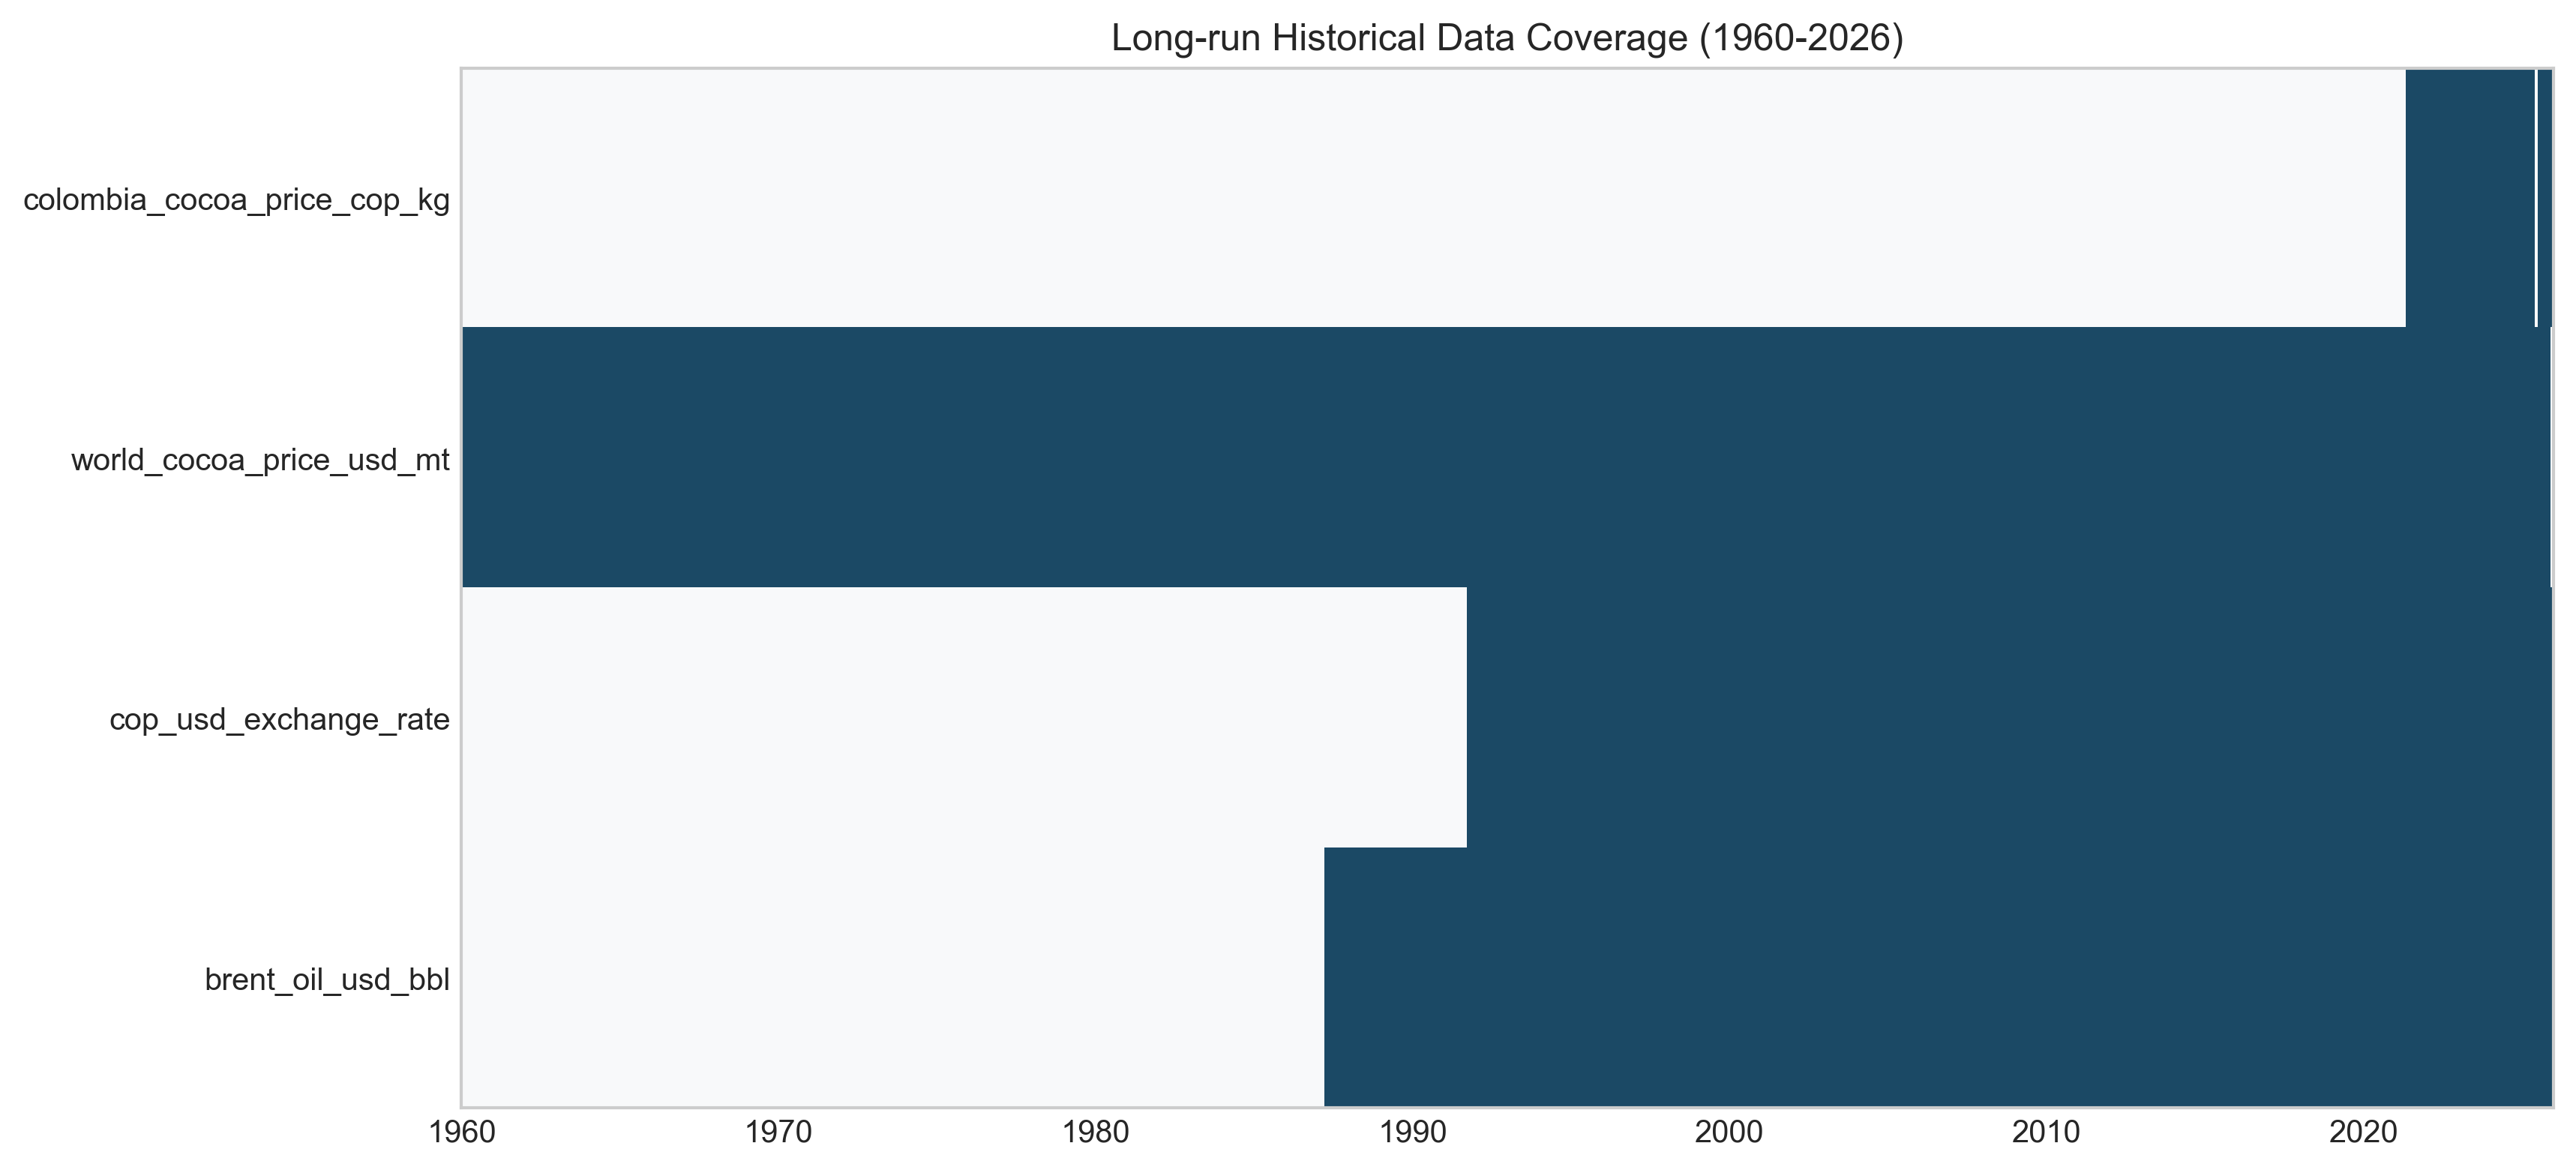
\includegraphics[keepaspectratio,alt={Figure 1. Long-run Historical Data Coverage (1960-2026).}]{figures/figure_v1_long_run_coverage.png}}
\caption{Figure 1. Long-run Historical Data Coverage (1960-2026).}
\end{figure}

\textbf{1.1 Long-run Connection Properties}

Analysis of the full historical sample reveals that domestic prices
internalize approximately \textbf{0.842} of world market shocks within
the same month. While Engle-Granger tests (p=0.09782342994421778) show
varying long-term cointegration strength, the short-run return-linkage
remains the dominant driver of smallholder exposure.

\textbf{Table 1. Core Transmission Benchmarks (V1 Metadata).}

{\def\LTcaptype{none} % do not increment counter
\begin{longtable}[]{@{}ll@{}}
\toprule\noalign{}
Metric & Value \\
\midrule\noalign{}
\endhead
\bottomrule\noalign{}
\endlastfoot
World-to-Domestic Pass-through & 0.842 \\
Model Adjusted R² & 0.633 \\
Engle-Granger p-value (Long-run) & 0.098 \\
Full Sample Observations & 55 \\
\end{longtable}
}

\subsection{Chapter 2: Territorial Hazard Dynamics in
Santander}\label{chapter-2-territorial-hazard-dynamics-in-santander}

The second layer identifies localized disaster pressure as an
exploratory contextual overlay. Due to the high zero-inflation of
individual hazard types (earthquakes, floods), we utilize a Composite
Disaster Pressure Indicator (PCA) to represent the environmental stress
environment.

\begin{figure}
\centering
\pandocbounded{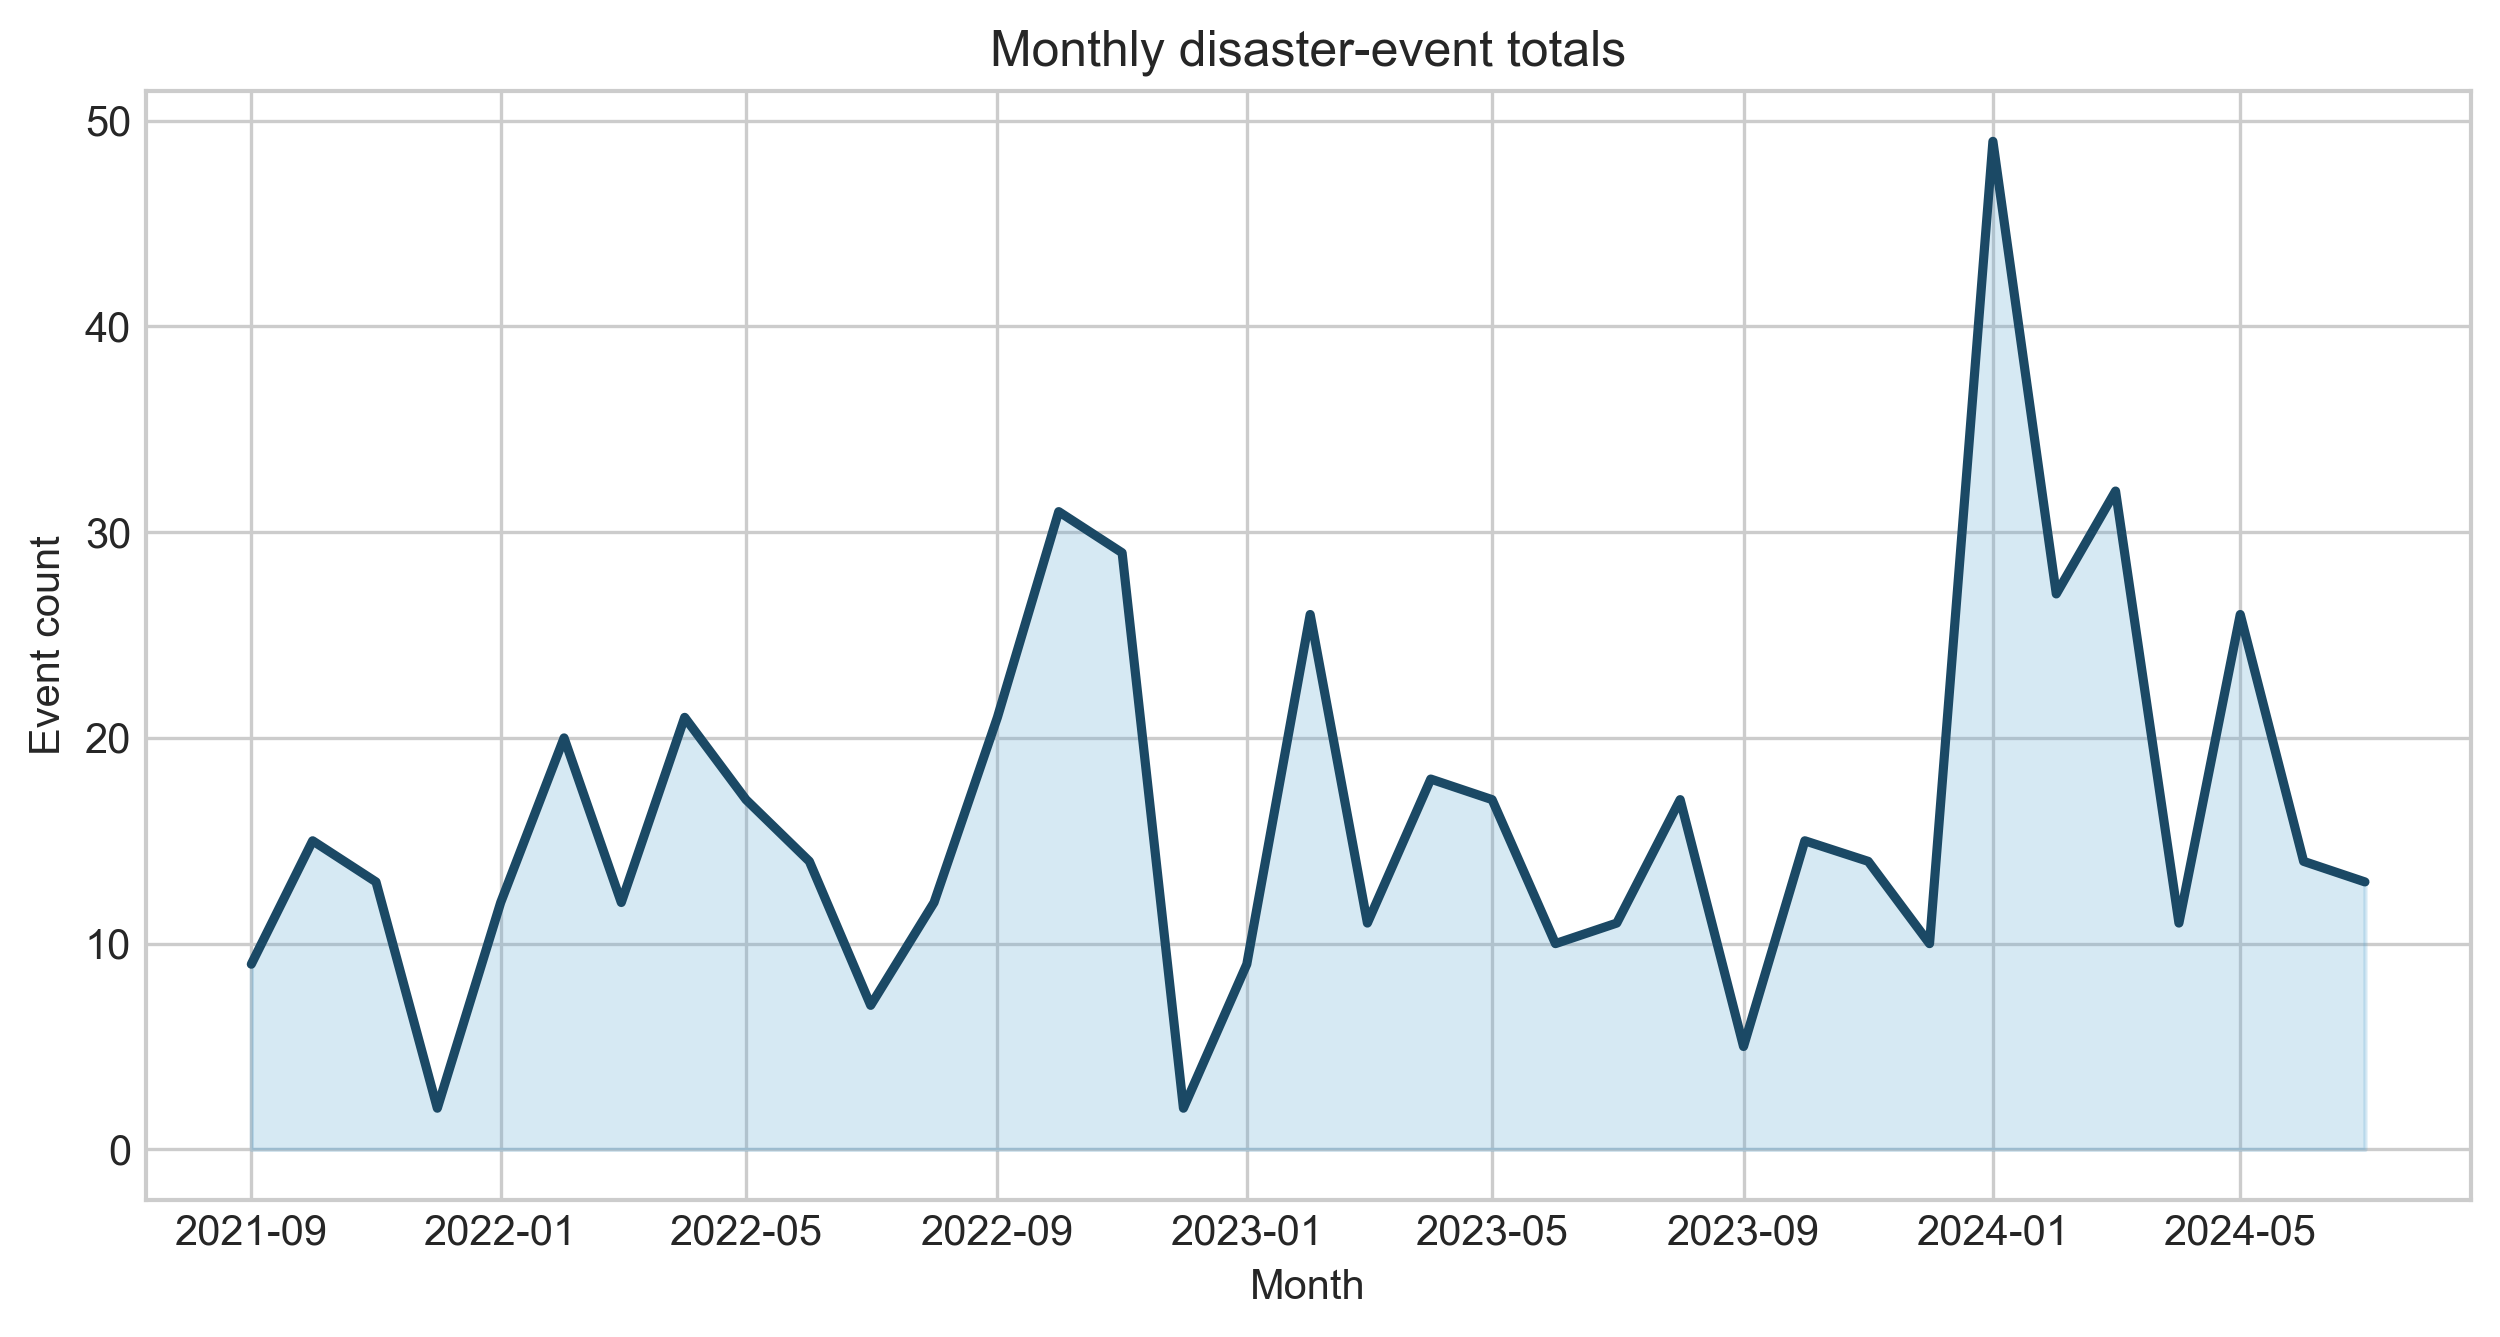
\includegraphics[keepaspectratio,alt={Figure 2. Monthly disaster-event totals.}]{figures/figure_monthly_event_totals.png}}
\caption{Figure 2. Monthly disaster-event totals.}
\end{figure}

\begin{figure}
\centering
\pandocbounded{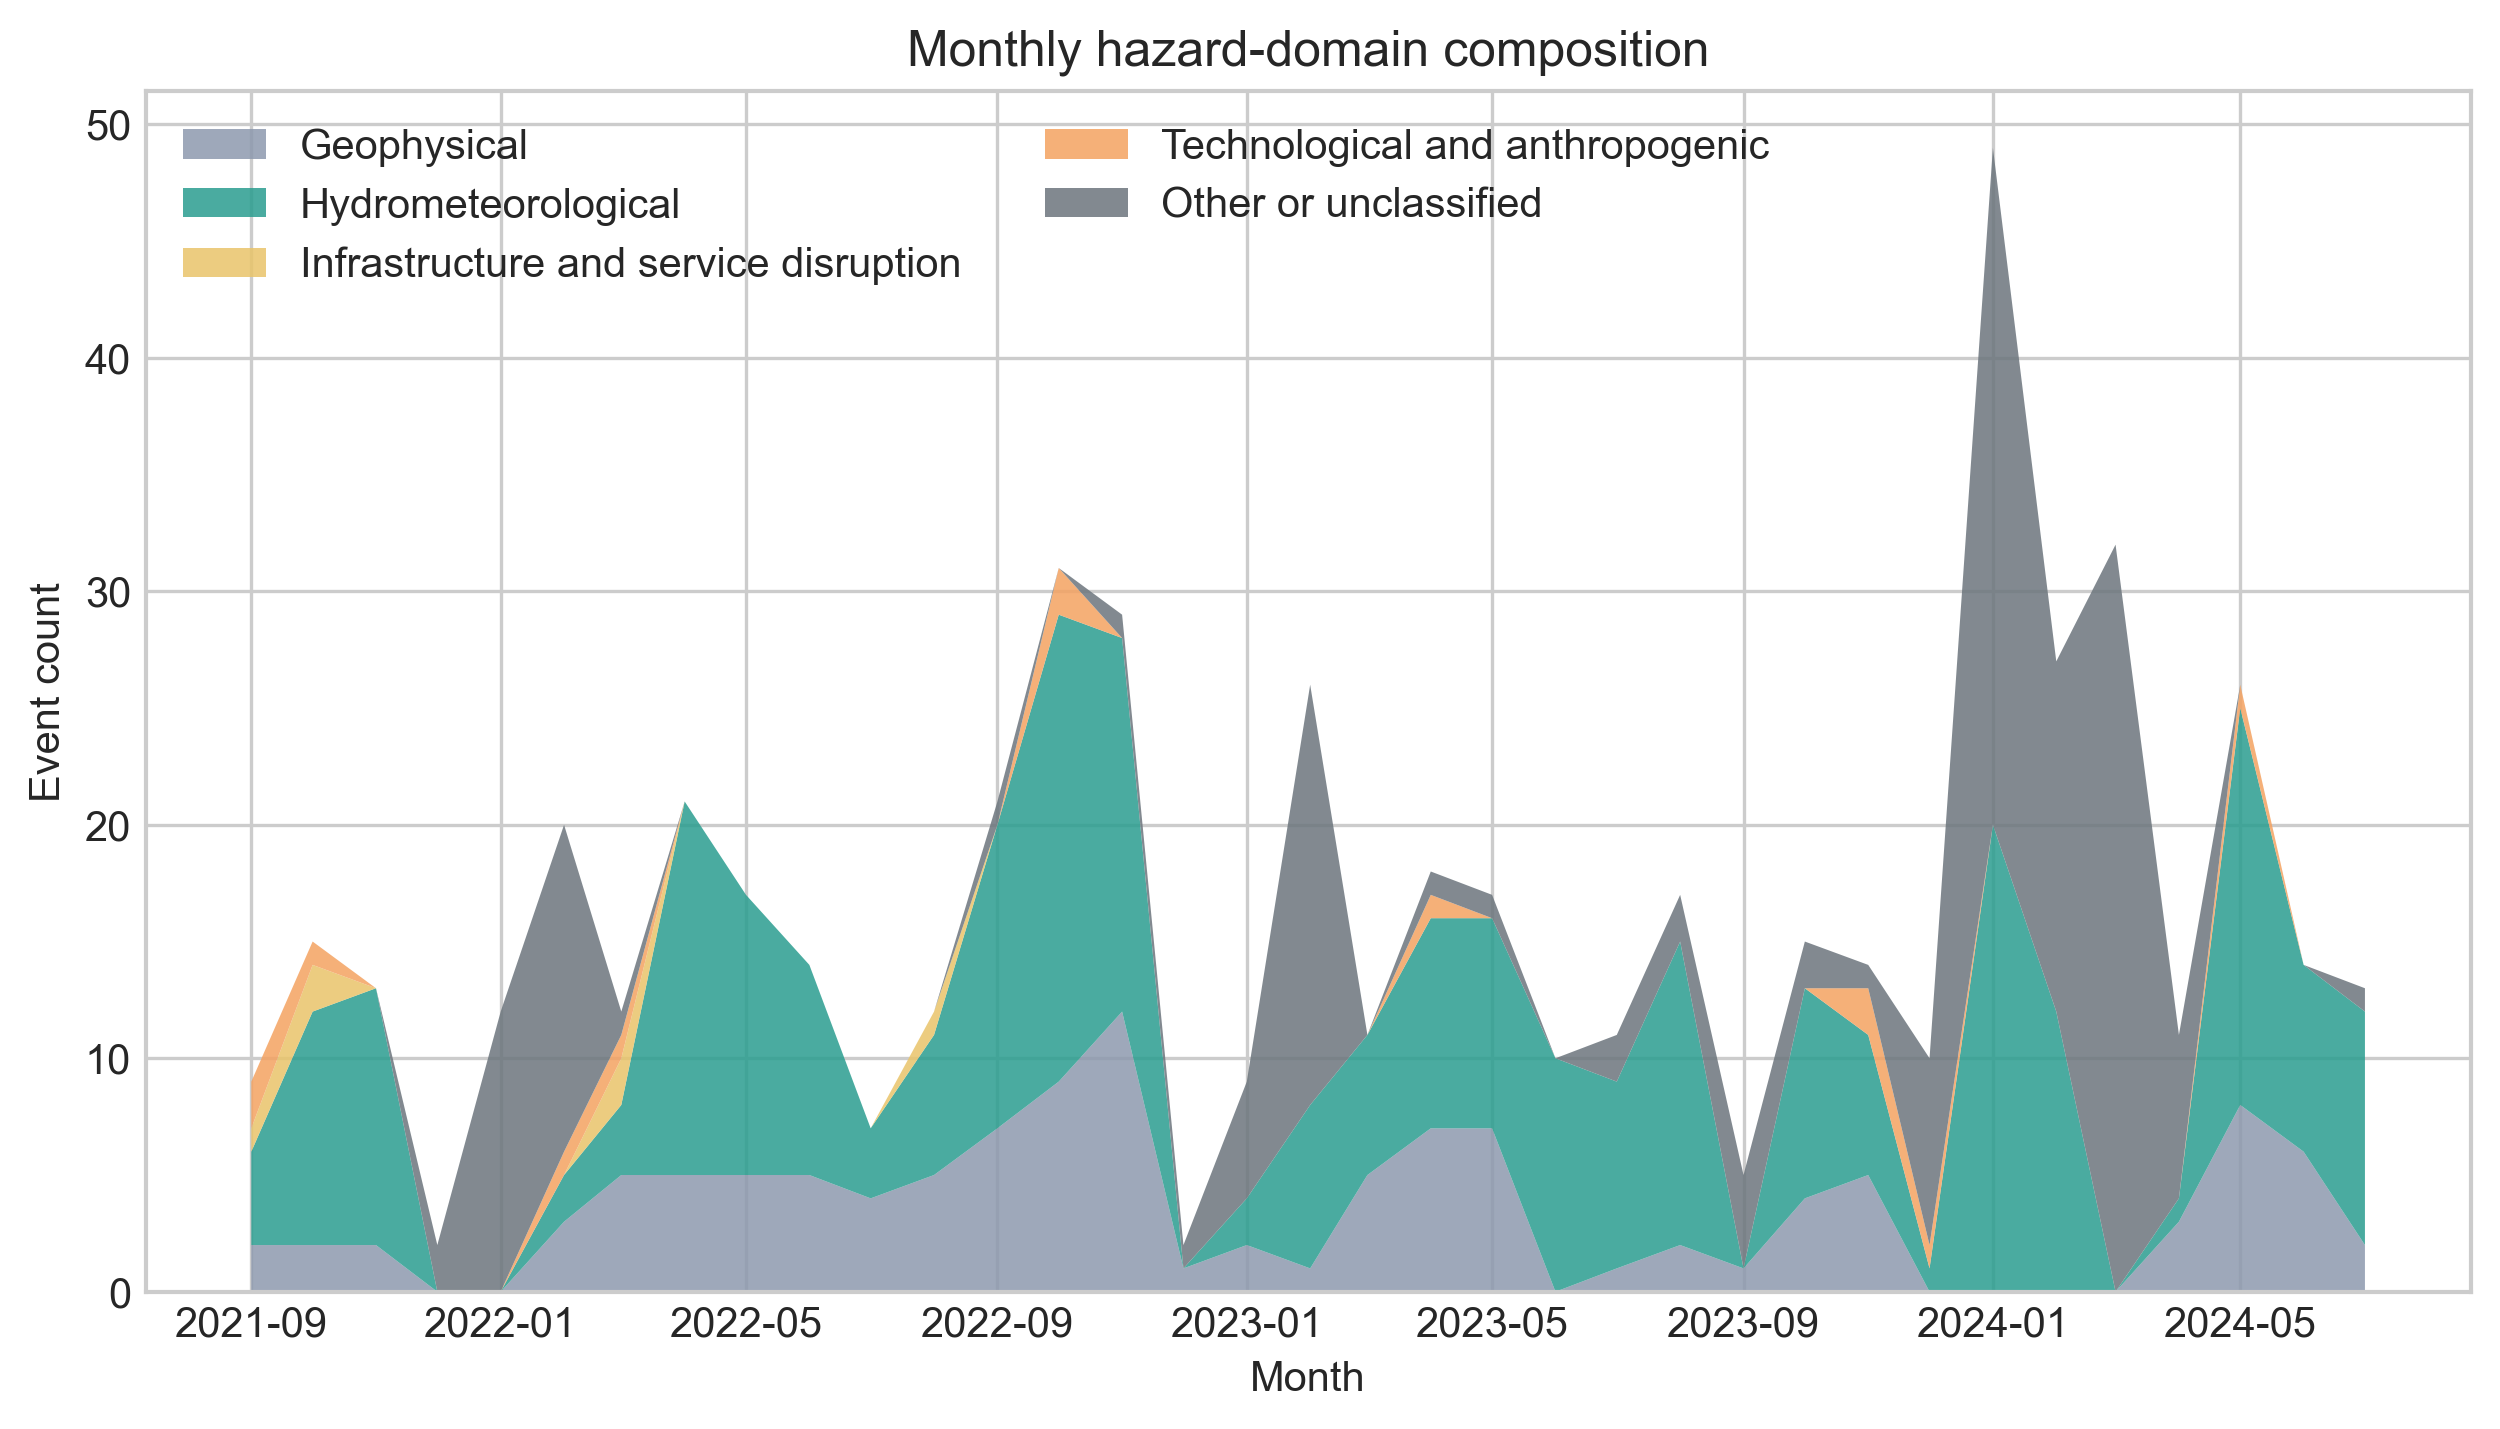
\includegraphics[keepaspectratio,alt={Figure 3. Monthly hazard-domain composition.}]{figures/figure_hazard_domain_mix.png}}
\caption{Figure 3. Monthly hazard-domain composition.}
\end{figure}

\textbf{Table 2. Aligned Sample configuration (Nested Disaster
Sub-window).}

{\def\LTcaptype{none} % do not increment counter
\begin{longtable}[]{@{}ll@{}}
\toprule\noalign{}
metric & value \\
\midrule\noalign{}
\endhead
\bottomrule\noalign{}
\endlastfoot
Source rows & 594 \\
Months in observation window & 36 \\
Date range start & 2021-08-01 \\
Date range end & 2024-07-30 \\
Distinct municipalities & 91 \\
Distinct event types & 25 \\
Earthquake-related events & 4 \\
\end{longtable}
}

\section{Chapter 3: Integrated Resilience Analytics
(Synthesis)}\label{chapter-3-integrated-resilience-analytics-synthesis}

When market shocks and disaster pressure are aligned, we observe the
intersection of price-taker risk and environmental vulnerability. Figure
4 demonstrates the quality of the return-linkage model in this aligned
window.

\begin{figure}
\centering
\pandocbounded{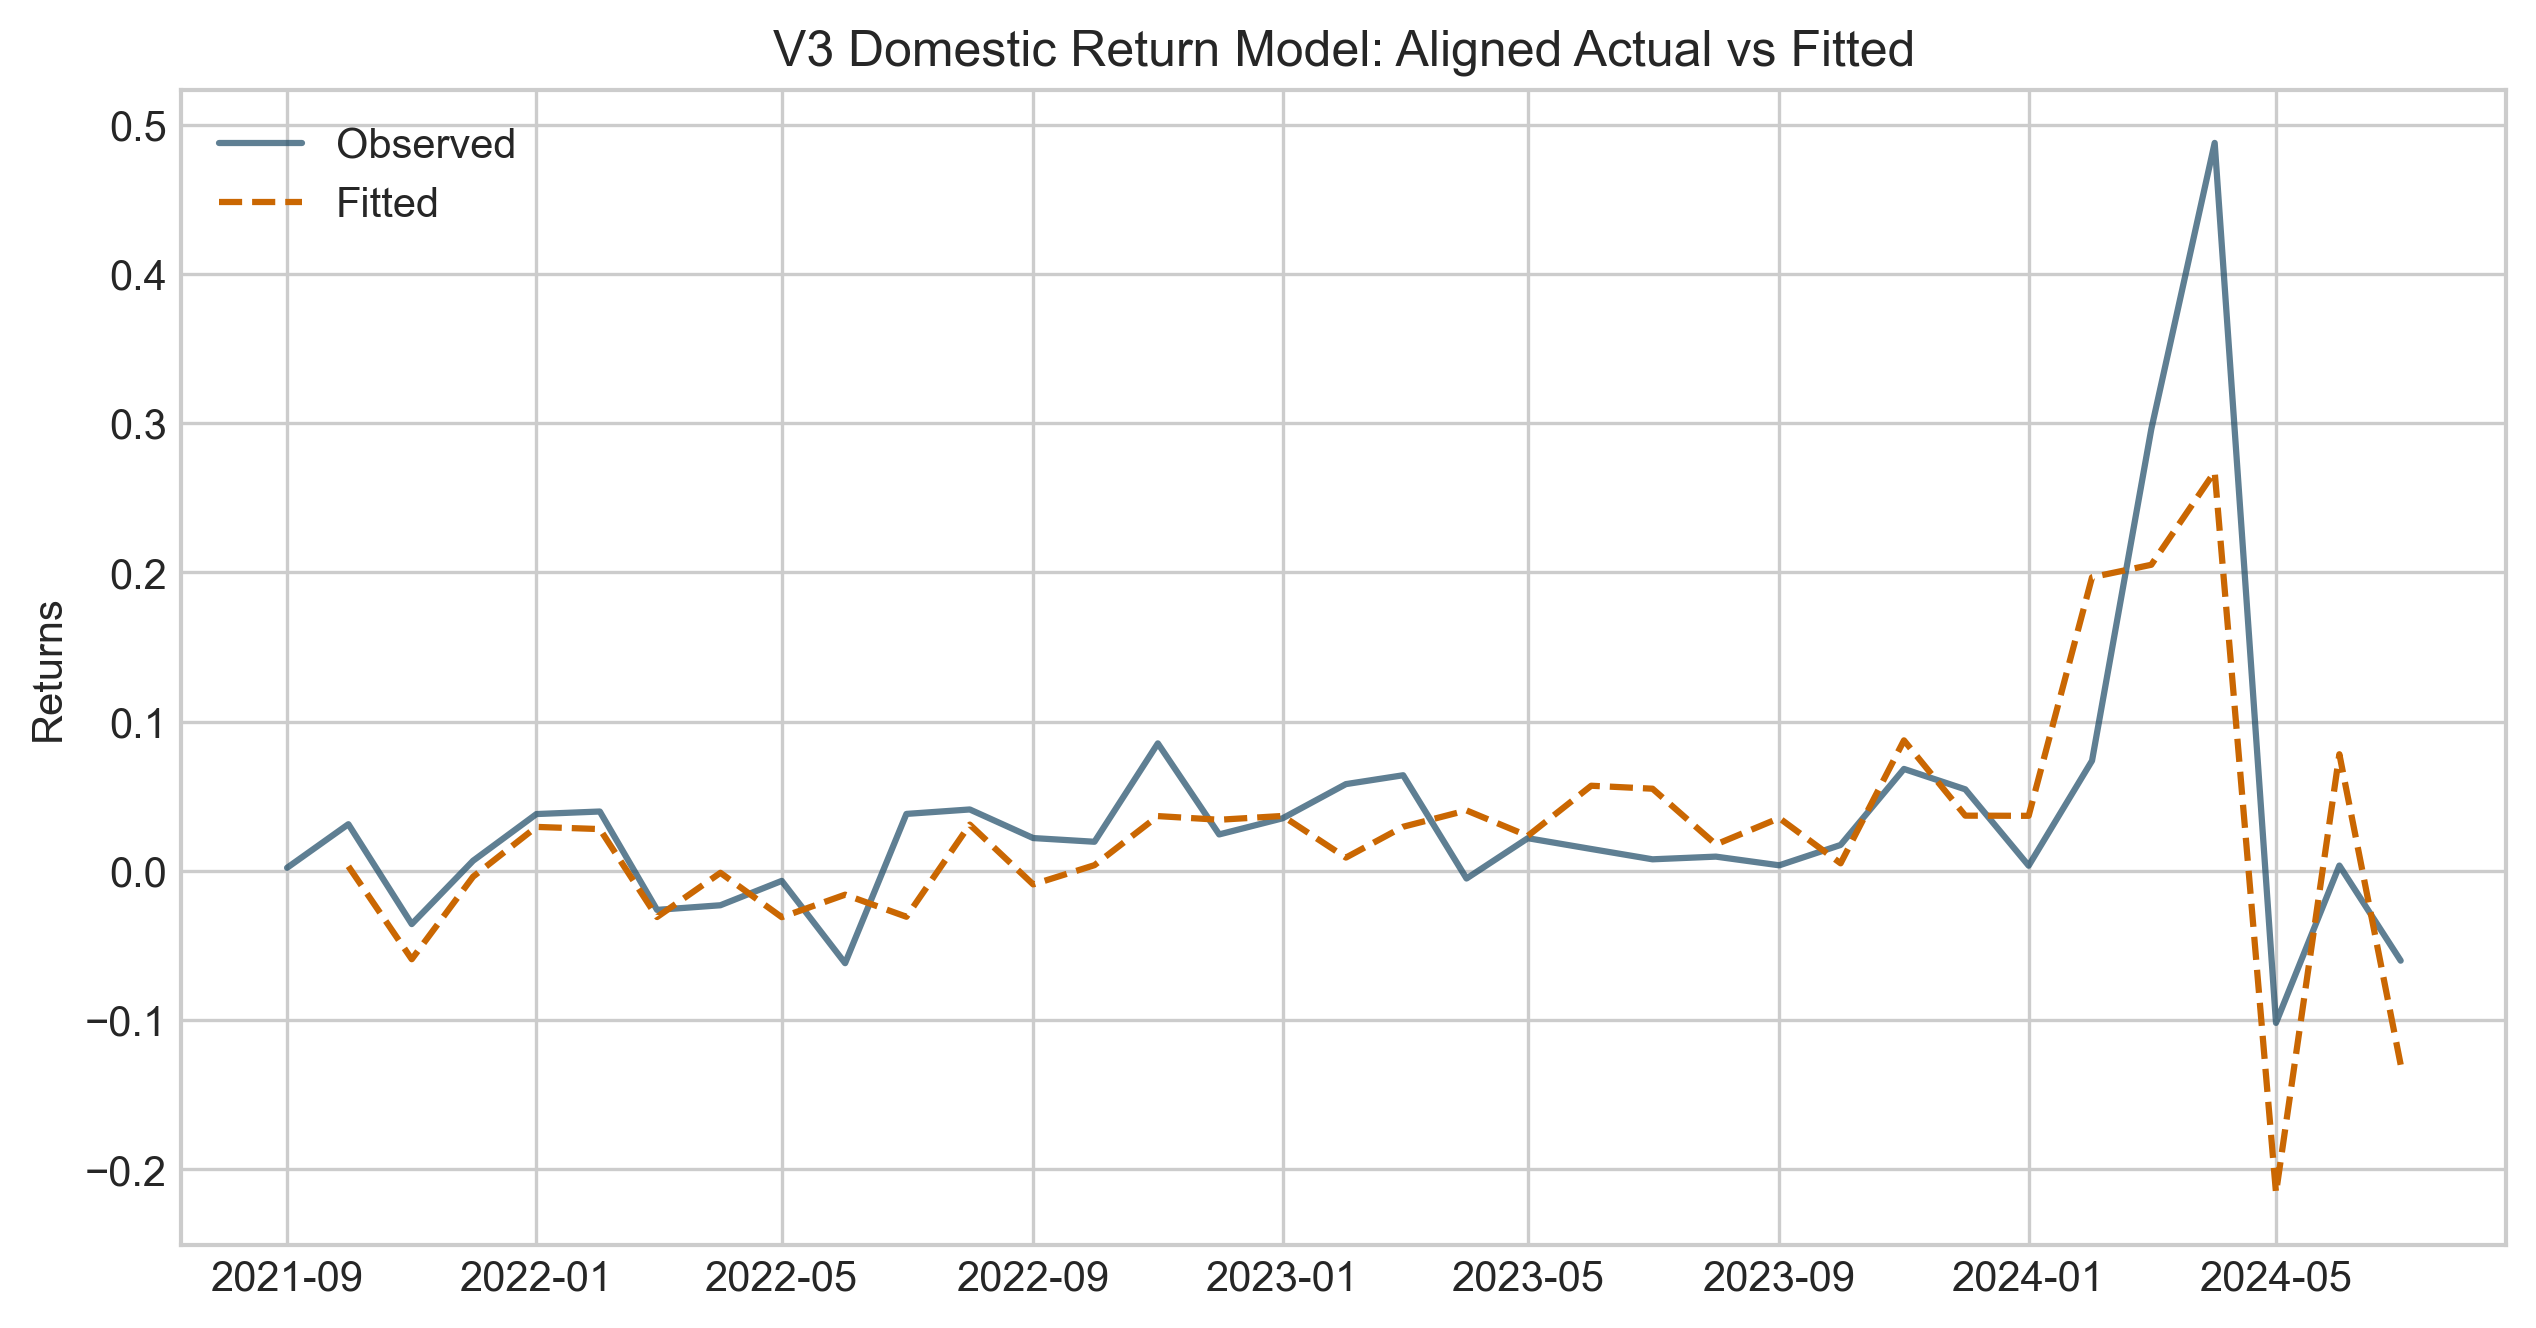
\includegraphics[keepaspectratio,alt={Figure 4. Aligned Return Model: Actual vs Fitted Analysis.}]{figures/figure_v3_actual_vs_fitted.png}}
\caption{Figure 4. Aligned Return Model: Actual vs Fitted Analysis.}
\end{figure}

\textbf{3.1 Systemic Granger Causality and Extensions}

Table 3 confirms that localized disaster pressure functions as a
contextual marker rather than a primary price setter. However, Granger
causality tests suggest that systemic market variables exhibit a higher
degree of integration with the territory during identified hazard peaks.

\textbf{Table 3. Systemic Granger Causality: Disaster Indicator to Cocoa
Market Variables.}

{\def\LTcaptype{none} % do not increment counter
\begin{longtable}[]{@{}
  >{\raggedright\arraybackslash}p{(\linewidth - 10\tabcolsep) * \real{0.1667}}
  >{\raggedright\arraybackslash}p{(\linewidth - 10\tabcolsep) * \real{0.1667}}
  >{\raggedright\arraybackslash}p{(\linewidth - 10\tabcolsep) * \real{0.1667}}
  >{\raggedright\arraybackslash}p{(\linewidth - 10\tabcolsep) * \real{0.1667}}
  >{\raggedright\arraybackslash}p{(\linewidth - 10\tabcolsep) * \real{0.1667}}
  >{\raggedright\arraybackslash}p{(\linewidth - 10\tabcolsep) * \real{0.1667}}@{}}
\toprule\noalign{}
\begin{minipage}[b]{\linewidth}\raggedright
source
\end{minipage} & \begin{minipage}[b]{\linewidth}\raggedright
target
\end{minipage} & \begin{minipage}[b]{\linewidth}\raggedright
lag
\end{minipage} & \begin{minipage}[b]{\linewidth}\raggedright
f\_statistic
\end{minipage} & \begin{minipage}[b]{\linewidth}\raggedright
p\_value
\end{minipage} & \begin{minipage}[b]{\linewidth}\raggedright
causal
\end{minipage} \\
\midrule\noalign{}
\endhead
\bottomrule\noalign{}
\endlastfoot
disaster\_indicator & colombia\_cocoa\_price\_cop\_kg\_log\_return & 1 &
0.025 & 0.876 & No \\
disaster\_indicator & colombia\_cocoa\_price\_cop\_kg\_log\_return & 2 &
0.013 & 0.987 & No \\
disaster\_indicator & colombia\_cocoa\_price\_cop\_kg\_log\_return & 3 &
0.053 & 0.983 & No \\
disaster\_indicator & colombia\_cocoa\_price\_cop\_kg\_log\_return & 4 &
0.138 & 0.967 & No \\
disaster\_indicator & world\_return & 1 & 0.205 & 0.654 & No \\
disaster\_indicator & world\_return & 2 & 0.043 & 0.958 & No \\
disaster\_indicator & world\_return & 3 & 0.096 & 0.961 & No \\
disaster\_indicator & world\_return & 4 & 0.445 & 0.775 & No \\
disaster\_indicator & fx\_return & 1 & 0.604 & 0.443 & No \\
disaster\_indicator & fx\_return & 2 & 0.274 & 0.762 & No \\
disaster\_indicator & fx\_return & 3 & 0.293 & 0.83 & No \\
disaster\_indicator & fx\_return & 4 & 0.789 & 0.545 & No \\
disaster\_indicator & oil\_return & 1 & 0.784 & 0.383 & No \\
disaster\_indicator & oil\_return & 2 & 0.565 & 0.575 & No \\
disaster\_indicator & oil\_return & 3 & 0.514 & 0.677 & No \\
disaster\_indicator & oil\_return & 4 & 0.66 & 0.627 & No \\
\end{longtable}
}

\textbf{3.2 The Disaster Overlay Models}

Model extensions (Table 4 and 5) show that while the disaster indicator
remains a restrained predictor in continuous space, it captures discrete
mean-shift episodes (Welch p=0.043) that mark periods of intensified
market stress.

\textbf{Table 4. Return Model Extension (Synthesized Disaster Overlay).}

{\def\LTcaptype{none} % do not increment counter
\begin{longtable}[]{@{}llll@{}}
\toprule\noalign{}
term & coefficient & std\_error & p\_value \\
\midrule\noalign{}
\endhead
\bottomrule\noalign{}
\endlastfoot
const & 0.011 & 0.007 & 0.116 \\
world\_return & 0.842 & 0.222 & 0 \\
fx\_return & 0.408 & 0.223 & 0.068 \\
oil\_return & -0.049 & 0.058 & 0.391 \\
disaster\_indicator & -0.001 & 0.002 & 0.562 \\
\end{longtable}
}

\textbf{Table 5. Volatility Model Extension (Synthesized Disaster
Overlay).}

{\def\LTcaptype{none} % do not increment counter
\begin{longtable}[]{@{}lll@{}}
\toprule\noalign{}
term & coefficient & p\_value \\
\midrule\noalign{}
\endhead
\bottomrule\noalign{}
\endlastfoot
const & 0.033 & 0 \\
world\_volatility & 2.842 & 0 \\
disaster\_indicator & -0.001 & 0.388 \\
\end{longtable}
}

\subsection{Chapter 4: Synthesis and Territorial Governance
Discussion}\label{chapter-4-synthesis-and-territorial-governance-discussion}

\subsubsection{4.1 Smallholder Vulnerability and `Farmer
Exposure'}\label{smallholder-vulnerability-and-farmer-exposure}

The synthesized findings introduce the \textbf{Farmer Exposure Index}
(Mean: 0.61). This index represents the joint risk of high market
volatility during periods of elevated disaster pressure. Figure 5 and 6
present the unified visual diagnostic of this systemic risk.

\begin{figure}
\centering
\pandocbounded{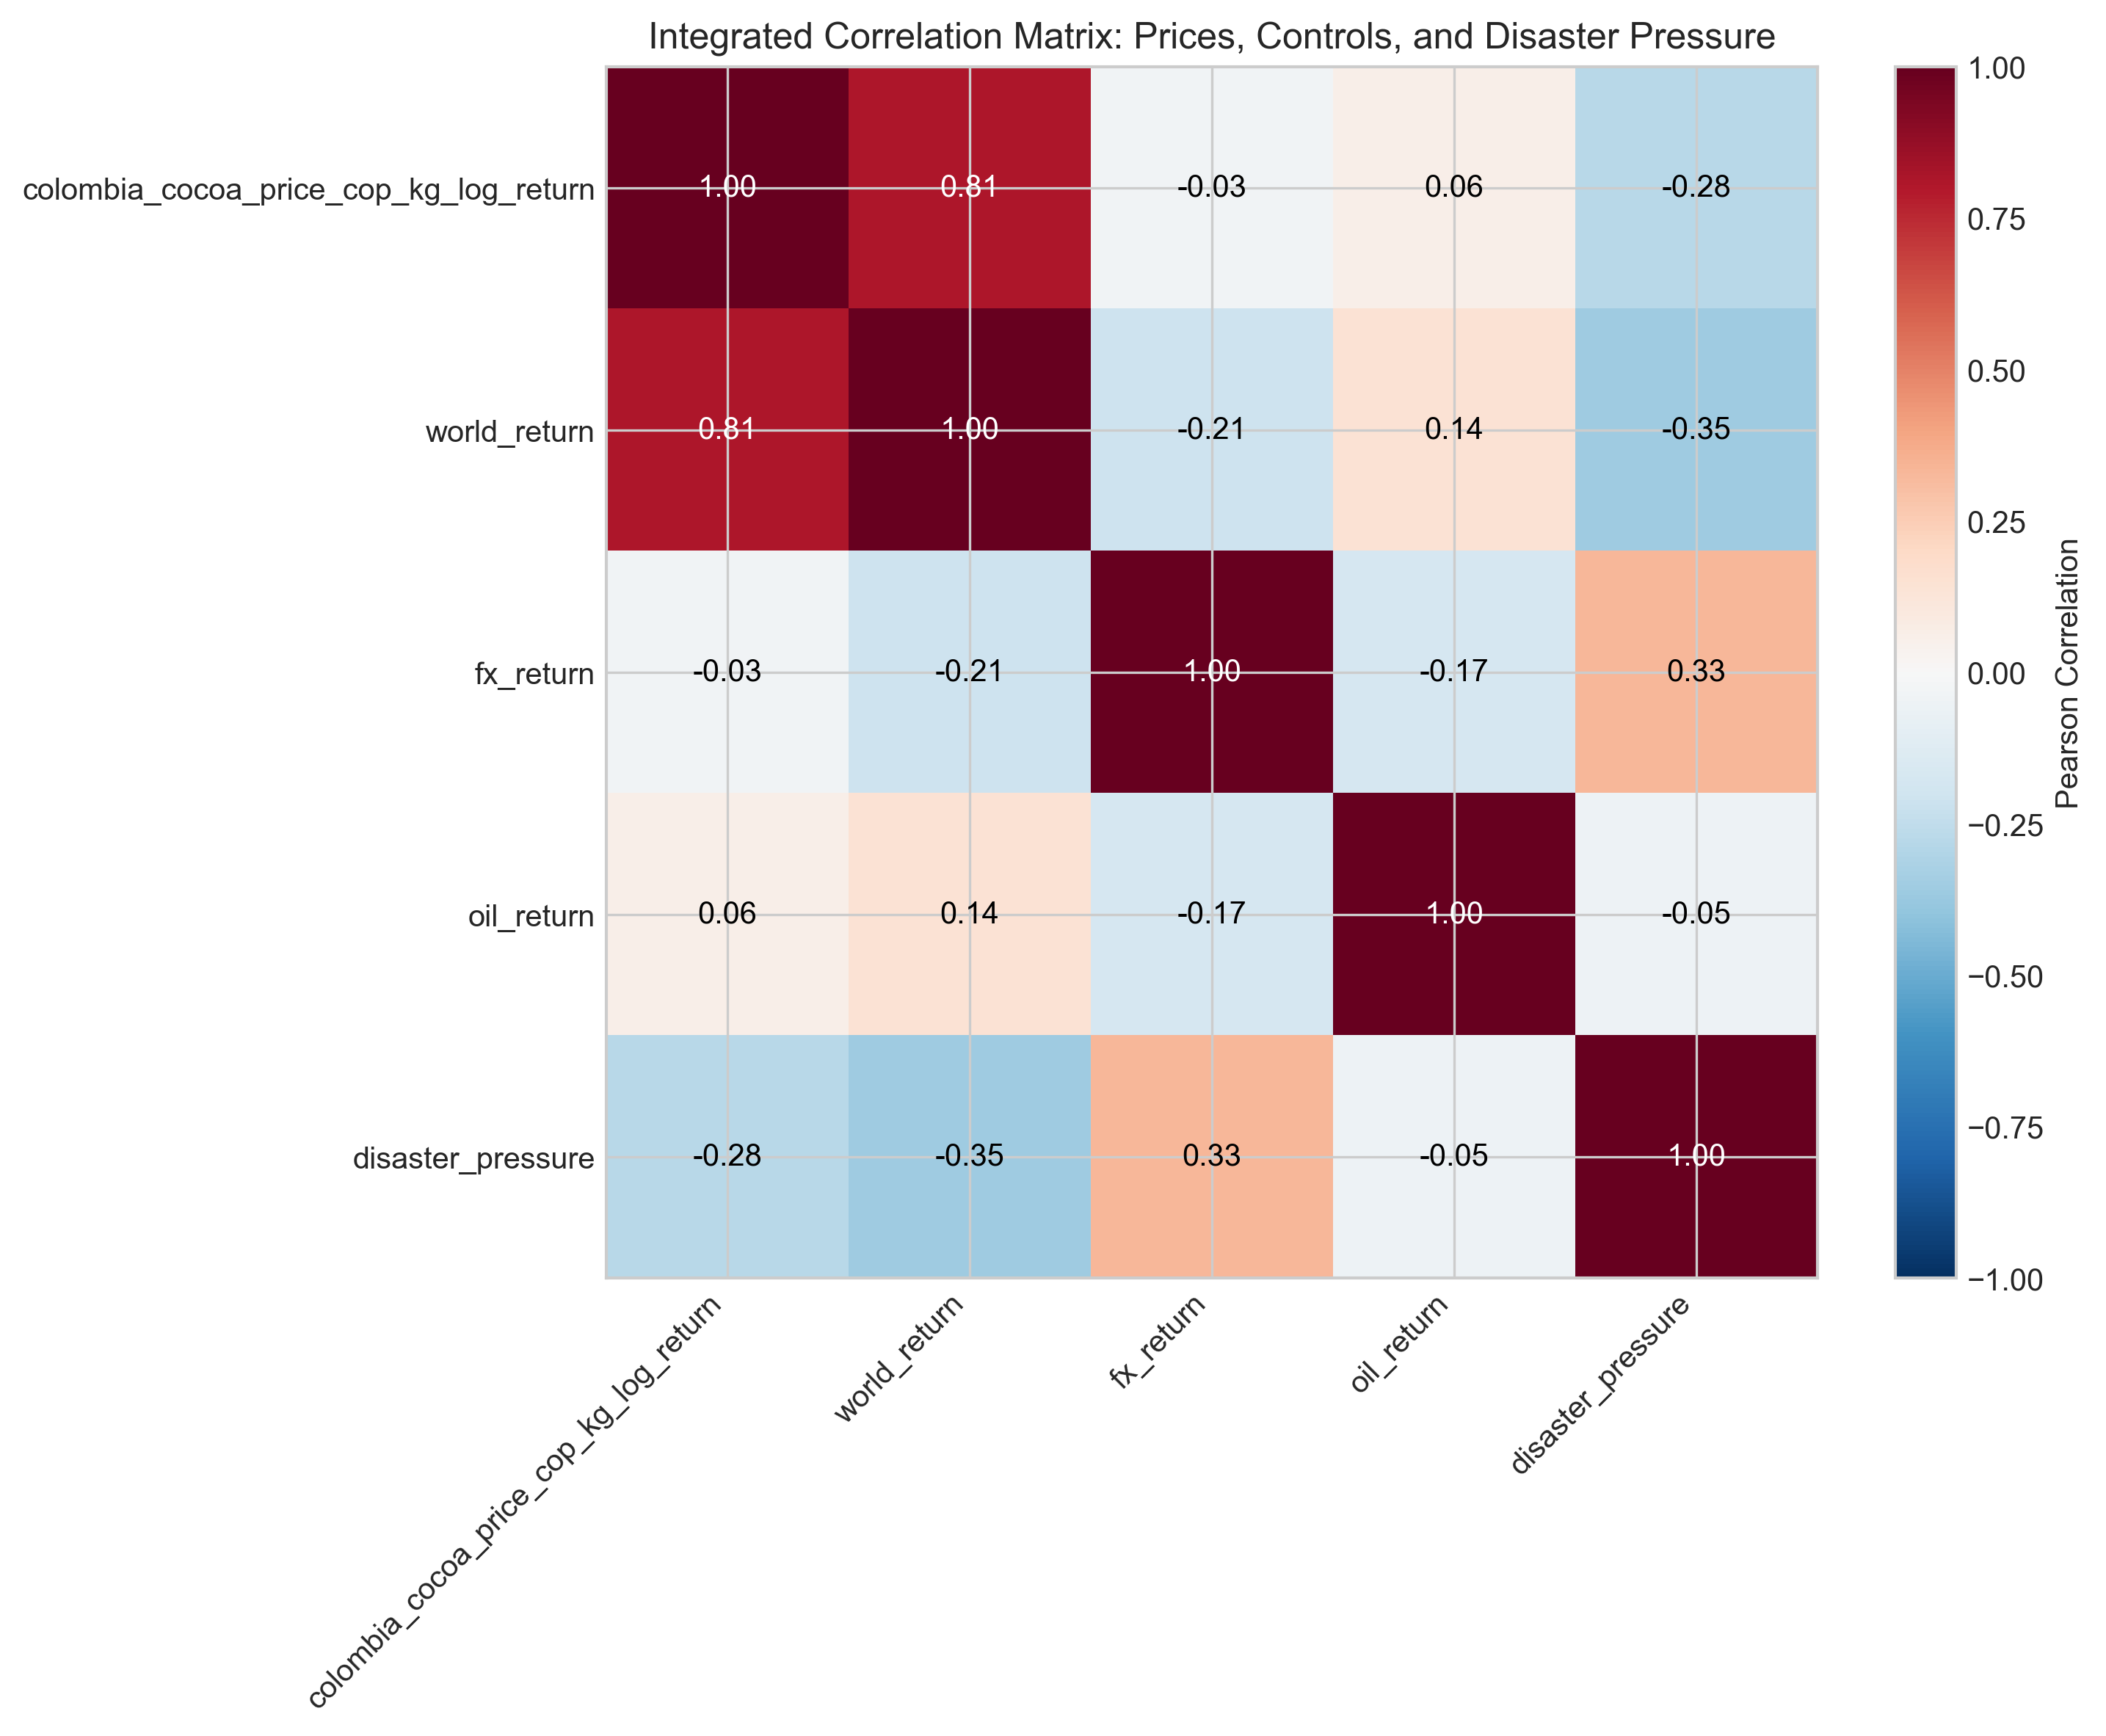
\includegraphics[keepaspectratio,alt={Figure 5. Integrated Correlation Matrix (Market + Risk).}]{figures/figure_v3_integrated_heatmap.png}}
\caption{Figure 5. Integrated Correlation Matrix (Market + Risk).}
\end{figure}

\begin{figure}
\centering
\pandocbounded{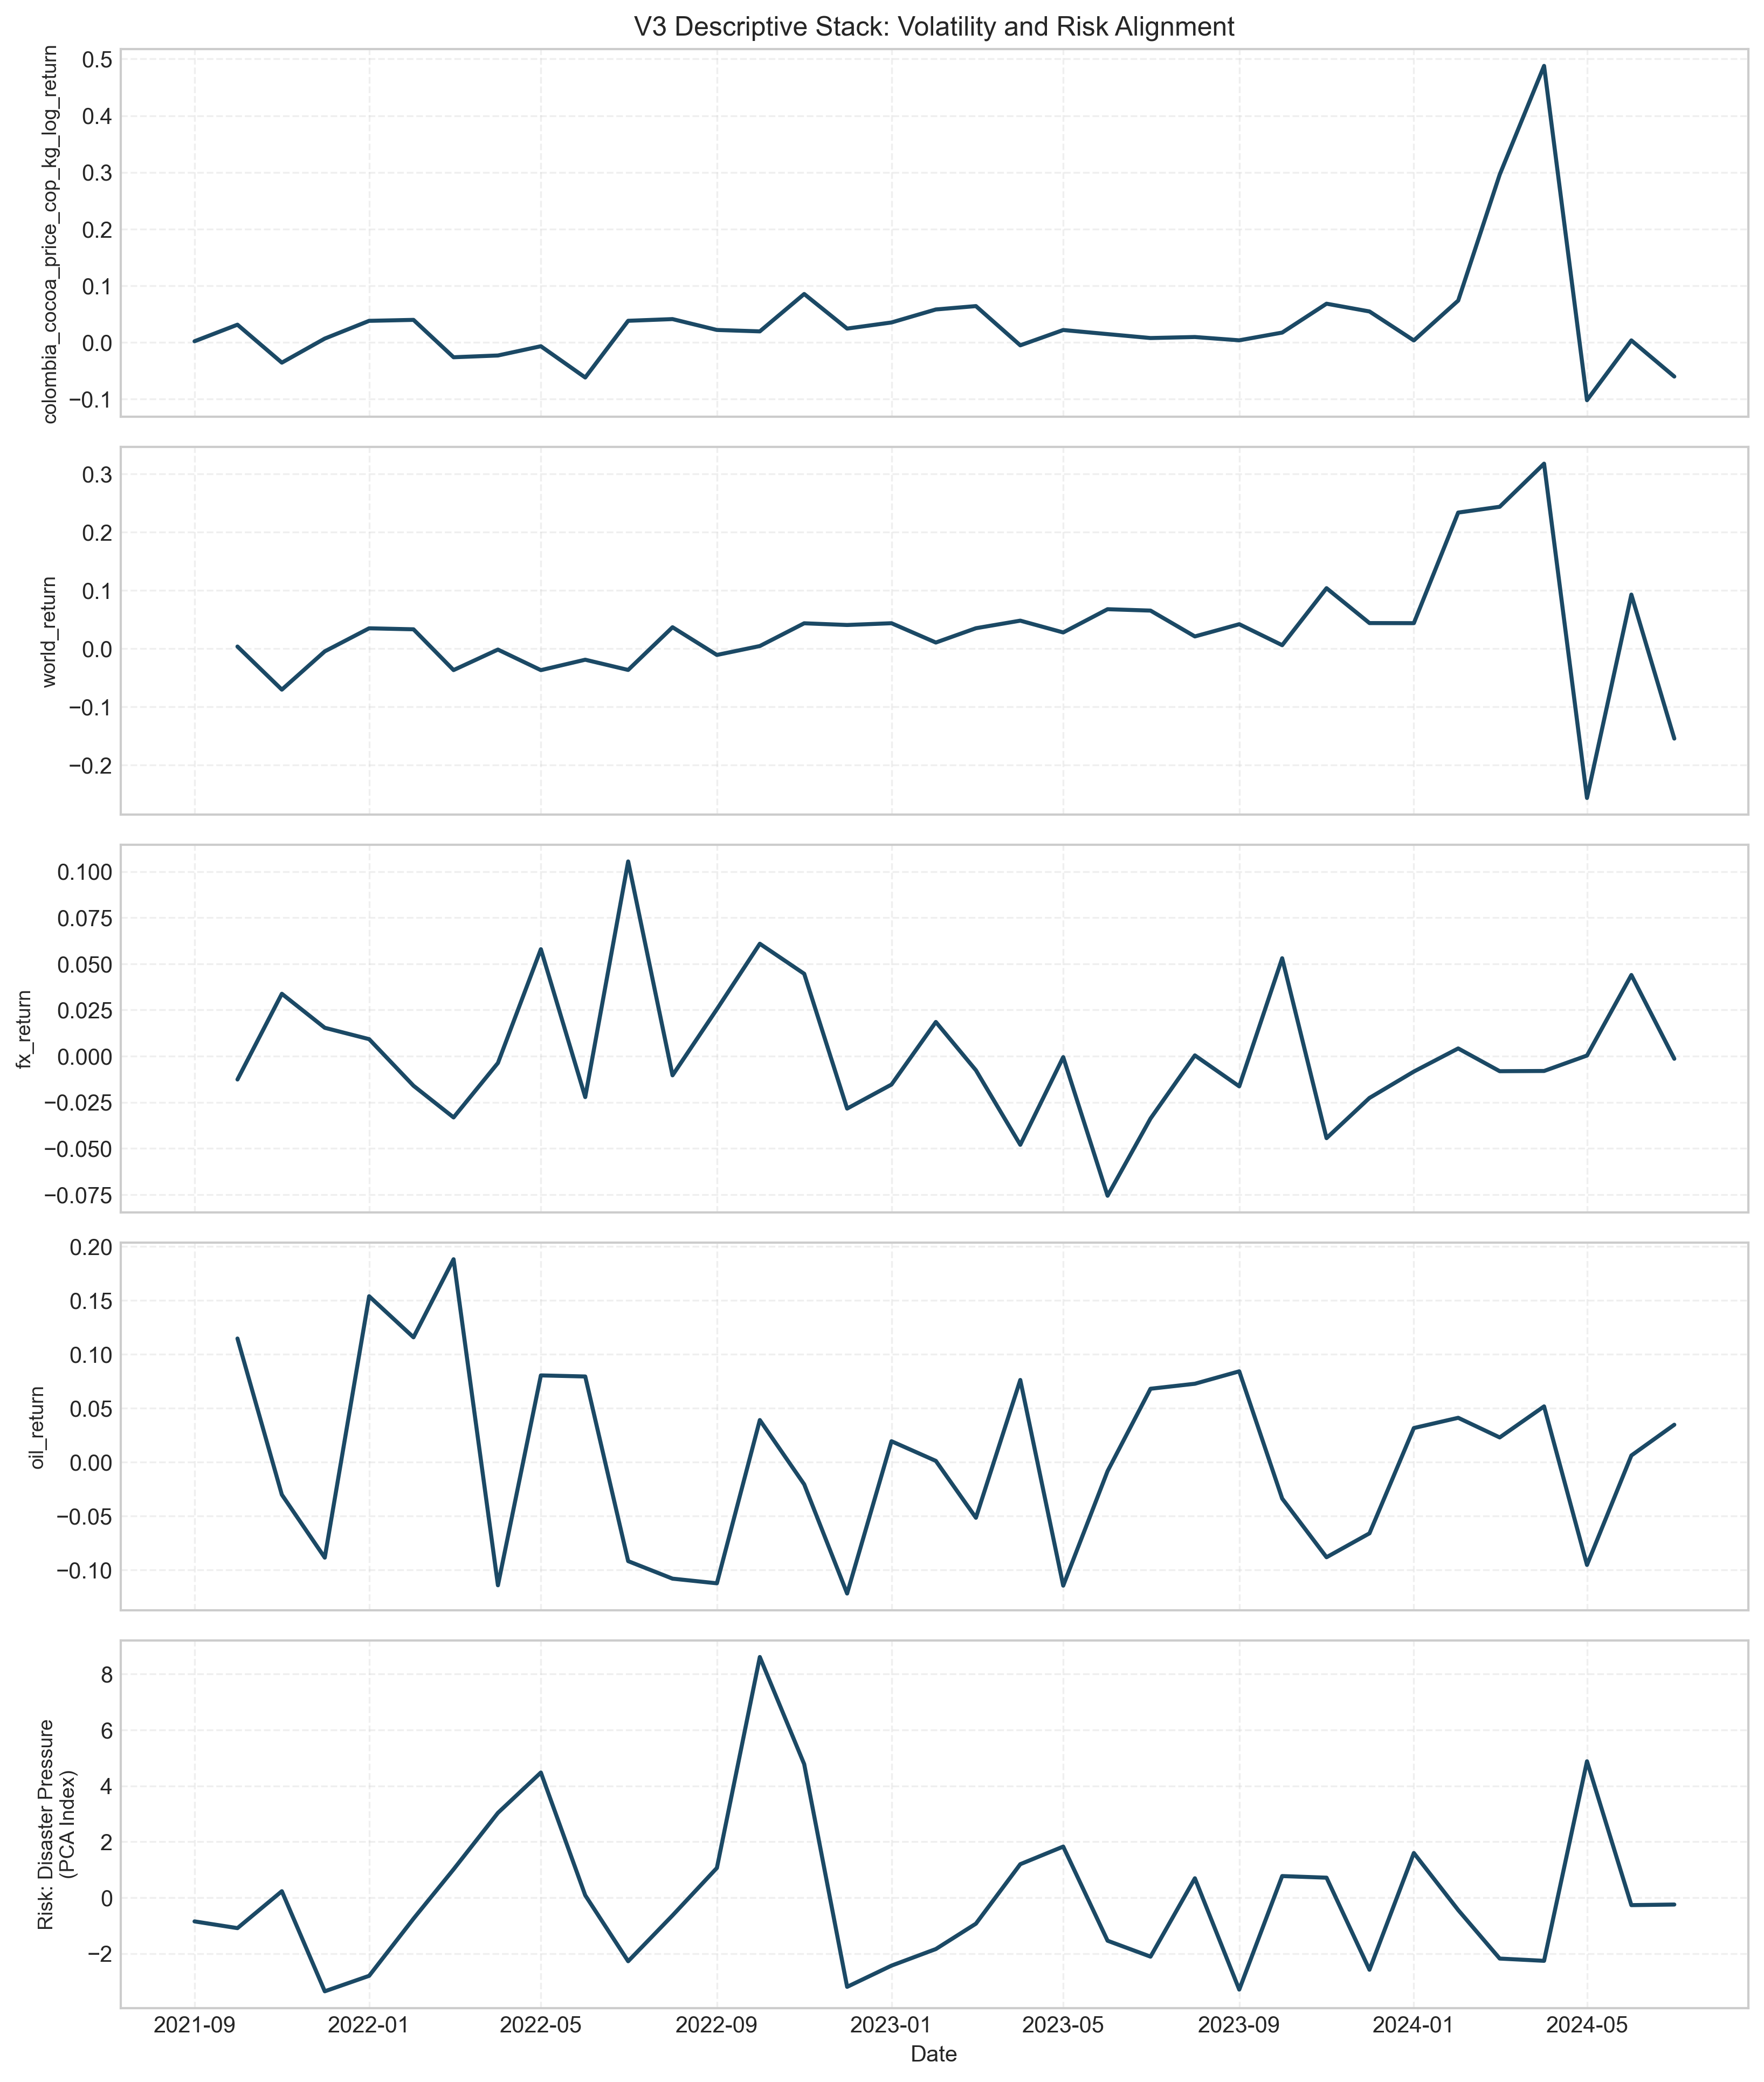
\includegraphics[keepaspectratio,alt={Figure 6. V3 Information Figures (Integrated Descriptive Views).}]{figures/figure_v3_descriptive_stack.png}}
\caption{Figure 6. V3 Information Figures (Integrated Descriptive
Views).}
\end{figure}

\subsubsection{4.2 Enriched Interpretation: Resilience as Buffer
Capacity}\label{enriched-interpretation-resilience-as-buffer-capacity}

The identification of natural hazards as \textbf{contextual amplifiers}
has significant implications for territorial governance. Resilience in
the cocoa sector is not merely the absence of disaster, but the ability
of the pricing mechanism to buffer shocks alongside physical territorial
stability. The coincidence of disaster peaks with market-level shifts
suggests that territorial risk can exacerbate the `price-taker' burden
of smallholders. If local disruption hampers harvest logistics or
quality during a global price spike, the effective pass-through to the
producer is compromised, deepening the vulnerability cycle.

\section{Appendix: Municipality Detail and Technical
Diagnostics}\label{appendix-municipality-detail-and-technical-diagnostics}

The following figures provide lower-level diagnostics for the
territorial hazard record.

\begin{figure}
\centering
\pandocbounded{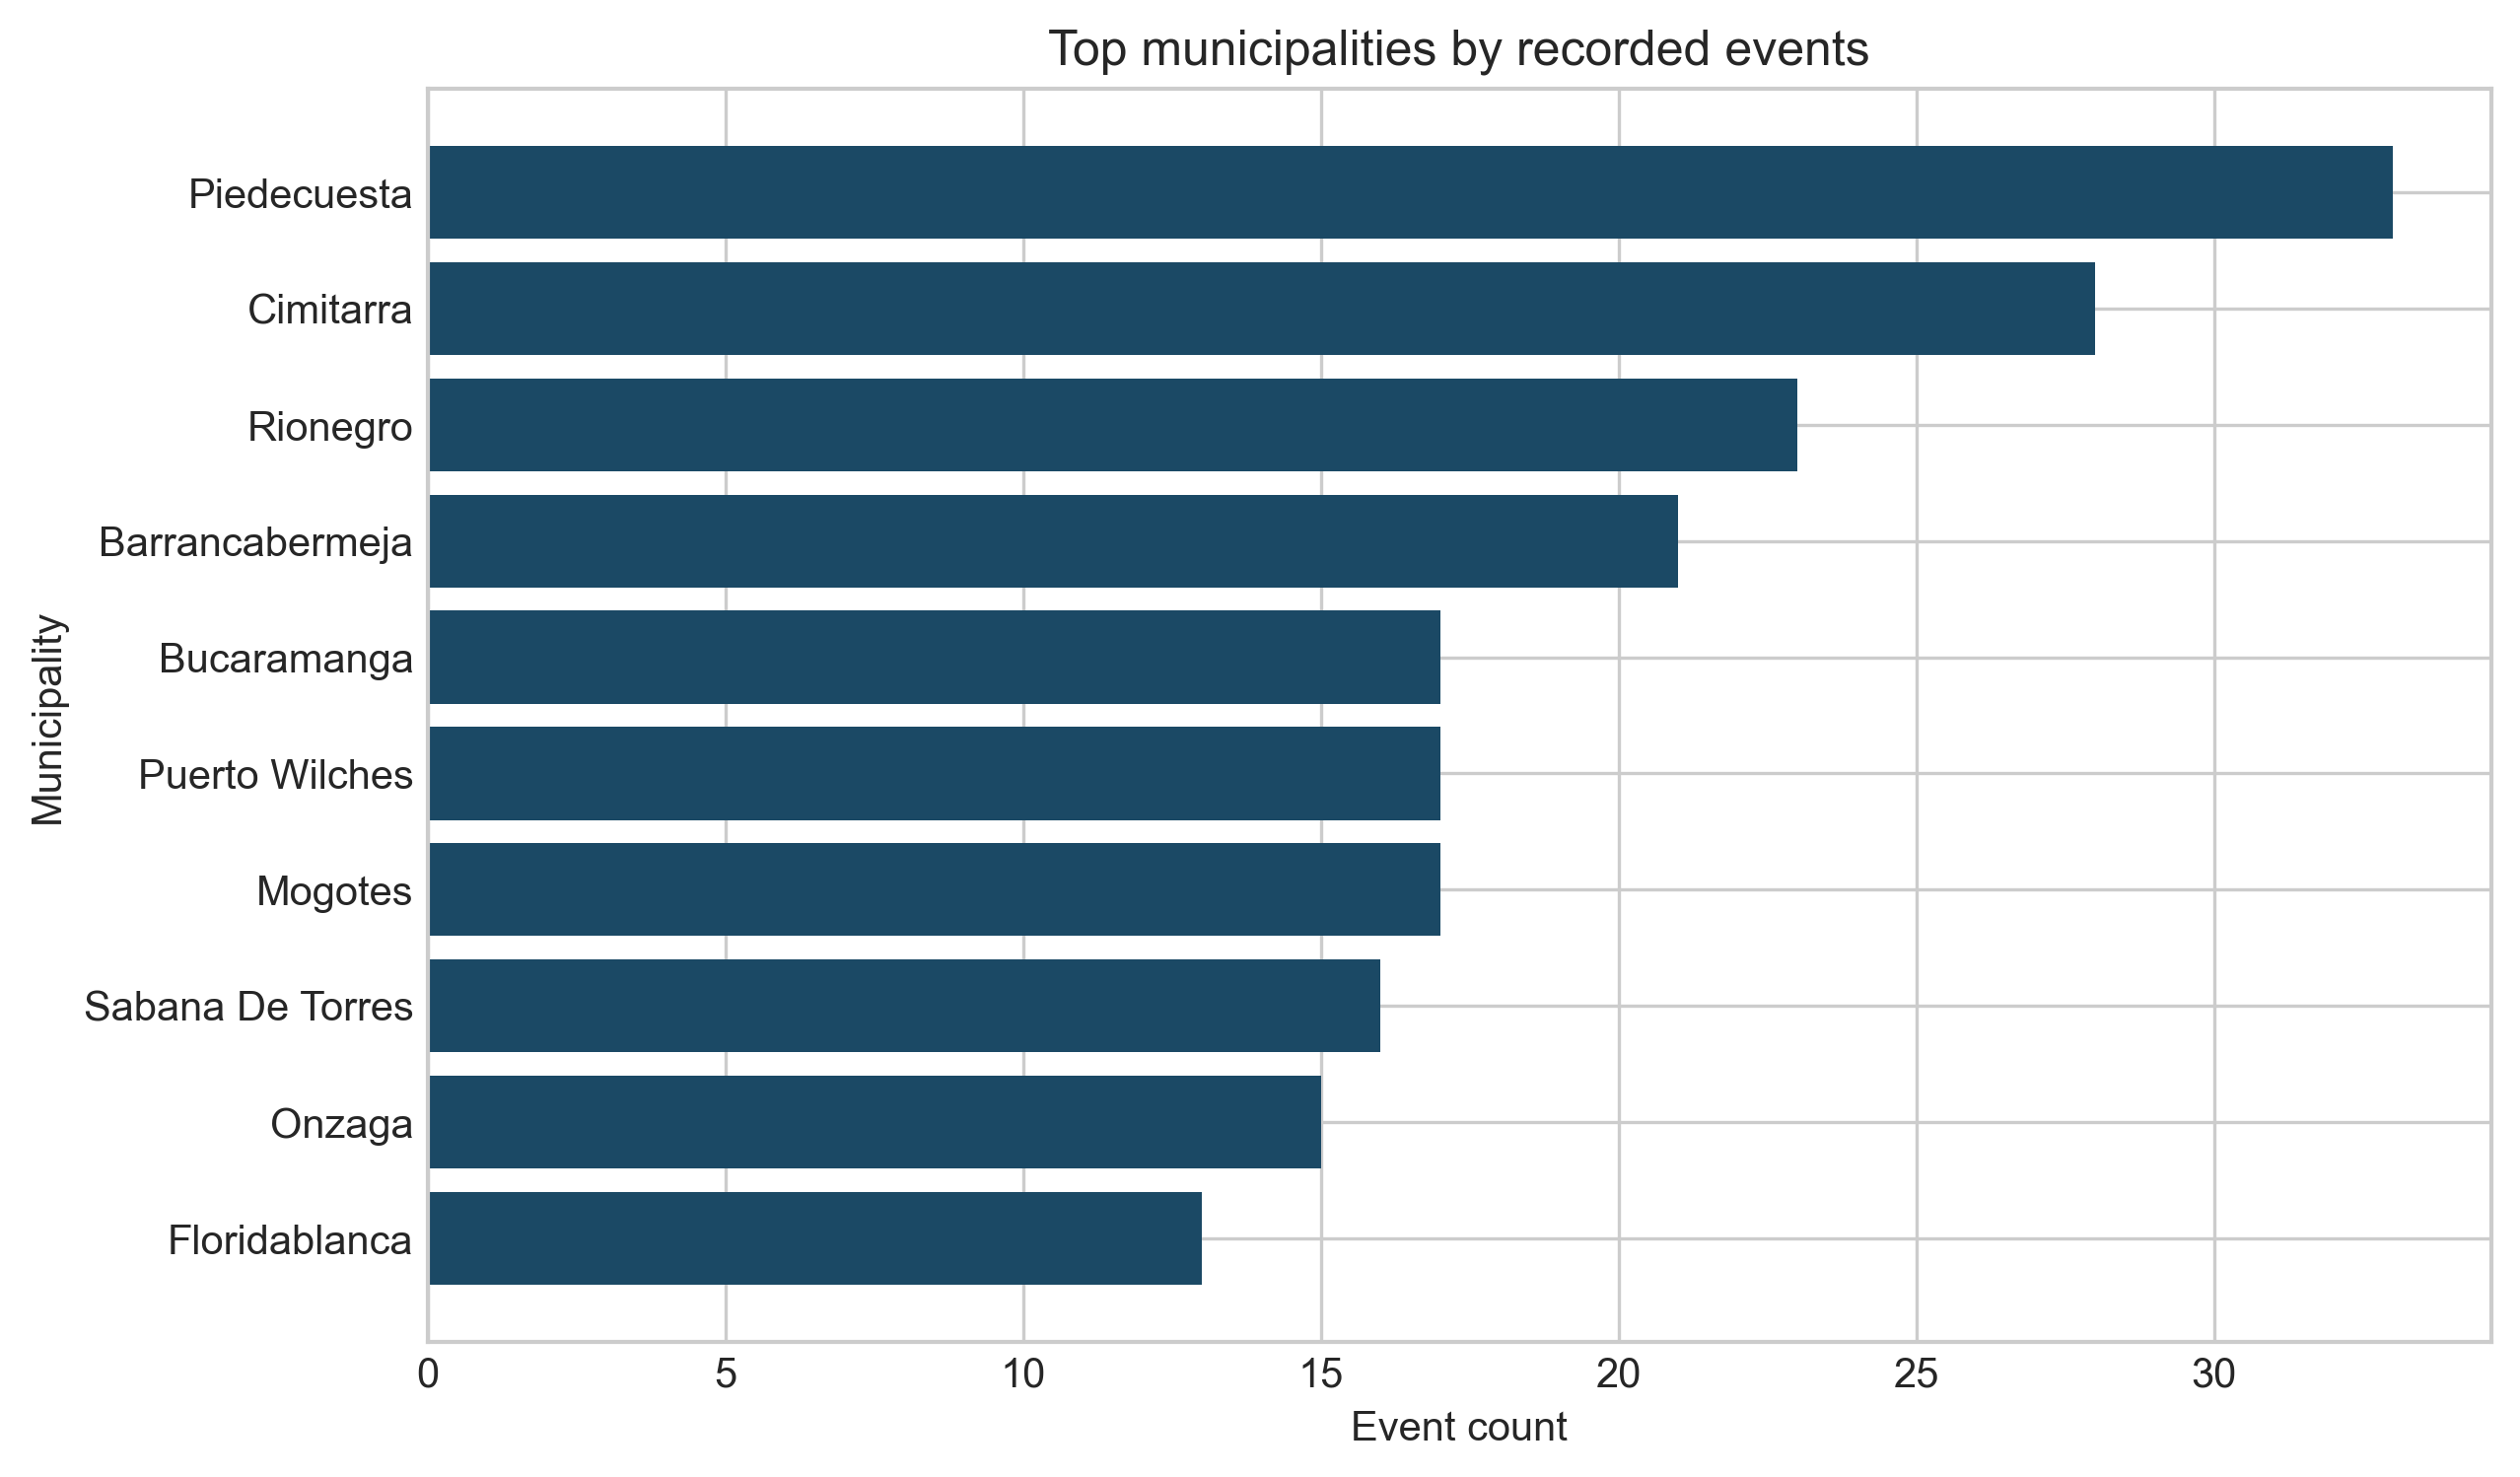
\includegraphics[keepaspectratio,alt={Figure A1. Top municipalities by recorded events.}]{figures/figure_top_municipalities.png}}
\caption{Figure A1. Top municipalities by recorded events.}
\end{figure}

\textbf{Table A1. Hazard Feasibility and Integration Checks.}

{\def\LTcaptype{none} % do not increment counter
\begin{longtable}[]{@{}
  >{\raggedright\arraybackslash}p{(\linewidth - 12\tabcolsep) * \real{0.1429}}
  >{\raggedright\arraybackslash}p{(\linewidth - 12\tabcolsep) * \real{0.1429}}
  >{\raggedright\arraybackslash}p{(\linewidth - 12\tabcolsep) * \real{0.1429}}
  >{\raggedright\arraybackslash}p{(\linewidth - 12\tabcolsep) * \real{0.1429}}
  >{\raggedright\arraybackslash}p{(\linewidth - 12\tabcolsep) * \real{0.1429}}
  >{\raggedright\arraybackslash}p{(\linewidth - 12\tabcolsep) * \real{0.1429}}
  >{\raggedright\arraybackslash}p{(\linewidth - 12\tabcolsep) * \real{0.1429}}@{}}
\toprule\noalign{}
\begin{minipage}[b]{\linewidth}\raggedright
criterion
\end{minipage} & \begin{minipage}[b]{\linewidth}\raggedright
observed\_value
\end{minipage} & \begin{minipage}[b]{\linewidth}\raggedright
threshold
\end{minipage} & \begin{minipage}[b]{\linewidth}\raggedright
rule
\end{minipage} & \begin{minipage}[b]{\linewidth}\raggedright
passes
\end{minipage} & \begin{minipage}[b]{\linewidth}\raggedright
Metric
\end{minipage} & \begin{minipage}[b]{\linewidth}\raggedright
p-value
\end{minipage} \\
\midrule\noalign{}
\endhead
\bottomrule\noalign{}
\endlastfoot
Total aligned months & 35 & 24 & \textgreater= & Yes & NA & NA \\
Non-zero aligned months & 4 & 12 & \textgreater= & No & NA & NA \\
Total aligned earthquake events & 4 & 18 & \textgreater= & No & NA &
NA \\
NA & NA & NA & NA & NA & ADF level check (Stationarity) & 0.273 \\
NA & NA & NA & NA & NA & ADF return check & 0.472 \\
NA & NA & NA & NA & NA & ARCH-LM test (Variance clustering) & 0.937 \\
NA & NA & NA & NA & NA & Correlation with Cocoa Returns & -0.277 \\
NA & NA & NA & NA & NA & Correlation with Rolling Volatility & 0.015 \\
\end{longtable}
}

\section{Limitations}\label{limitations}

This synthesis is constrained by the 36-month overlap where
high-fidelity disaster records are available. The findings should be
treated as a reproducible methodology for vulnerability assessment
rather than as proof of permanent structural transitions.

\end{document}
